\documentclass[10pt, twocolumn]{article}
\usepackage[margin=0.75in]{geometry}
\usepackage{graphicx}
\usepackage{tikz}
\usepackage{pgfplots}
\usepackage{booktabs}
\usepackage{amsmath}
\usepackage{amssymb}
\usepackage{pifont}
\usepackage{algorithm}
\usepackage{algorithmic}
\usepackage{hyperref}
\usepackage{xcolor}
\usepackage{caption}
\usepackage{subcaption}
\usepackage{fancyhdr}
\usepackage{enumitem}
\usepackage{listings}
\usepackage{microtype}
\usepackage{orcidlink}
\usepackage{tabularx}
\usepackage{multirow}
\usepackage{xspace}
\pgfplotsset{compat=1.18}
\usetikzlibrary{arrows.meta, positioning, shapes.geometric, fit, calc, backgrounds, decorations.markings}

% Checkmark / cross shortcuts
\newcommand{\cmark}{\ding{51}\xspace}
\newcommand{\xmark}{\ding{55}\xspace}

% ORCID icon (inline TikZ)
\definecolor{orcidgreen}{HTML}{A6CE39}
\newcommand{\orcidicon}{%
  
\begin{tikzpicture}[baseline=(char.base)]
    \node[circle, fill=orcidgreen, inner sep=0pt, minimum size=2.2ex] (char)
      {\textcolor{white}{\sffamily\bfseries\scriptsize iD}};
  \end{tikzpicture}%
}

% Color palette (professional blues/teals/oranges — matches AgenticMemory paper)
\definecolor{aiblue}{HTML}{2563EB}
\definecolor{aidarkblue}{HTML}{1E40AF}
\definecolor{aiteal}{HTML}{0D9488}
\definecolor{aiorange}{HTML}{EA580C}
\definecolor{aigray}{HTML}{6B7280}
\definecolor{ailightgray}{HTML}{F3F4F6}
\definecolor{aigreen}{HTML}{059669}
\definecolor{aired}{HTML}{DC2626}
\definecolor{aipurple}{HTML}{7C3AED}

% Listings style
\lstset{
  basicstyle=\ttfamily\scriptsize,
  keywordstyle=\color{aiblue}\bfseries,
  commentstyle=\color{aigray}\itshape,
  stringstyle=\color{aiteal},
  breaklines=true,
  frame=single,
  rulecolor=\color{aigray!30},
  backgroundcolor=\color{ailightgray},
  numbers=left,
  numberstyle=\tiny\color{aigray},
  tabsize=2
}

% Header
\pagestyle{fancy}
\fancyhf{}
\renewcommand{\headrulewidth}{0.4pt}
\fancyhead[L]{\small\textit{AgenticIdentity}}
\fancyhead[R]{\small\thepage}

\title{\textbf{AgenticIdentity: A Cryptographic Trust Anchor\\for AI Agent Systems}}
\author{Omoshola Owolabi\,\orcidlink{0009-0006-4089-0732}\\Researcher -- AI/ML\\Agentra Labs\\\texttt{omoshola.owolabi@agentralabs.tech}}
\date{February 24, 2026}

\begin{document}
\maketitle
\thispagestyle{fancy}

% ============================================================================
% ABSTRACT
% ============================================================================
\begin{abstract}
Large language model agents increasingly take consequential actions---deploying code, sending messages, managing infrastructure---yet lack any cryptographic mechanism to prove identity, sign actions, or establish trust.
We present AgenticIdentity, a cryptographic trust anchor that gives AI agents persistent, portable, mathematically verifiable identity.
The system introduces three primitives: (1)~\emph{identity anchors} rooted in Ed25519 key pairs with hierarchical key derivation via HKDF-SHA256, (2)~\emph{action receipts} that produce signed, chainable, witness-attested proofs of every agent action, and (3)~a \emph{trust web} of signed, scoped, time-bounded, revocable, and delegatable capability grants with URI-based permission matching.
We implement AgenticIdentity in 10{,}859 lines of Rust across four crates---core library, CLI, MCP server, and C~FFI---with 182~tests and zero external service dependencies.
Benchmarks on Apple~M4~Pro show Ed25519 key generation in 8.80\,\textmu{}s, action signing in 11.55\,\textmu{}s, receipt verification in 21.77\,\textmu{}s, and trust chain verification (depth~2) in 43.51\,\textmu{}s---all sub-millisecond, enabling real-time use in interactive agent systems.
AgenticIdentity is the fourth module in AgenticOS, providing the cryptographic foundation upon which agent contracts, communication, and orchestration are built.
\end{abstract}

% ============================================================================
% 1. INTRODUCTION
% ============================================================================
\section{Introduction}
\label{sec:intro}

The transformer architecture~\cite{vaswani2017attention} has produced language models capable of tool use~\cite{schick2024toolformer}, multi-step reasoning~\cite{yao2023react}, and autonomous task execution~\cite{park2023generative}. Increasingly, these models operate as \emph{agents}---software entities that observe their environment, make decisions, and take actions with real-world consequences: deploying code, sending emails, modifying databases, and managing infrastructure.

Yet every AI agent today is \emph{anonymous}. When an agent takes an action, there is no cryptographic proof that \emph{this specific agent} performed \emph{this specific action}. Session identifiers vanish. API keys authenticate the human operator, not the agent. Logs can be tampered with. There is no mechanism for an agent to prove its identity to another agent, no way to grant an agent scoped permissions that can be revoked, and no portable identity that survives session boundaries or provider changes.

This creates four fundamental problems. \textbf{No accountability:} when something goes wrong, there is no chain of custody linking an action to an agent with mathematical certainty. \textbf{No trust delegation:} permissions are all-or-nothing API keys; there is no ``trust this agent to read my calendar but not my email, and revoke if compromised.'' \textbf{No agent-to-agent authentication:} when Agent~A receives a message from Agent~B, there is no proof B sent it. \textbf{No portability:} an agent's identity is trapped in one platform; switching providers means starting from zero.

We present AgenticIdentity, a cryptographic system that addresses all four problems through three primitives:

\begin{enumerate}[nosep, leftmargin=*]
  \item \textbf{Identity Anchors} --- Ed25519 key pairs where the public key \emph{is} the agent's identity, with hierarchical key derivation (HKDF-SHA256) for scoped session, capability, and device keys, plus key rotation without identity loss.
  \item \textbf{Action Receipts} --- Signed proofs of every action, with hash-chain links for tamper-evident audit trails and optional witness co-signatures for multi-party non-repudiation.
  \item \textbf{Trust Web} --- Signed, scoped, time-bounded, revocable trust grants with URI-based capability matching, delegation chains with depth limits, and configurable revocation channels.
\end{enumerate}

AgenticIdentity is the fourth module in the AgenticOS ecosystem~\cite{owolabi2026agenticmemory, owolabi2026agenticcodebase, owolabi2026agenticvision}, providing the cryptographic foundation upon which agent contracts, communication, and orchestration are built.

The remainder of this paper is organized as follows. Section~\ref{sec:background} surveys existing identity systems and their limitations for AI agents. Section~\ref{sec:architecture} presents the architecture in detail. Section~\ref{sec:implementation} describes the Rust implementation. Section~\ref{sec:evaluation} reports micro-benchmarks and security analysis. Section~\ref{sec:usecases} describes concrete use cases. Section~\ref{sec:related} discusses related work. Section~\ref{sec:conclusion} concludes.

% Figure 1: Problem illustration (full width)
\begin{figure*}[t]
\centering
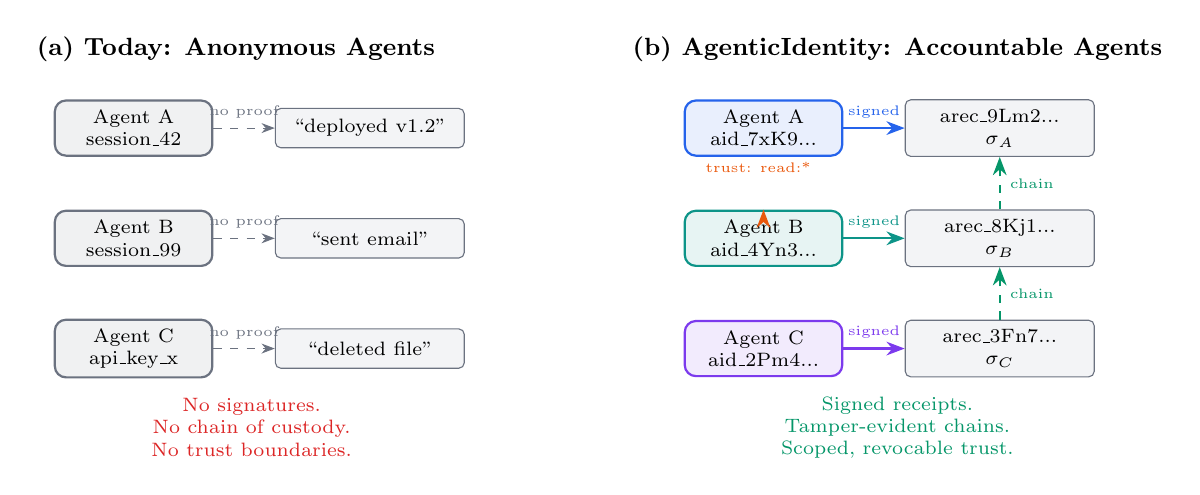
\begin{tikzpicture}[
  node distance=1.2cm,
  every node/.style={font=\small},
  agentbox/.style={rectangle, rounded corners=4pt, draw=#1, fill=#1!10, minimum width=2.0cm, minimum height=0.7cm, font=\scriptsize, align=center, thick},
  actionbox/.style={rectangle, rounded corners=2pt, draw=aigray, fill=ailightgray, minimum width=2.4cm, minimum height=0.5cm, font=\scriptsize, align=center},
  badlabel/.style={font=\scriptsize\color{aired}, align=center},
  goodlabel/.style={font=\scriptsize\color{aigreen}, align=center},
]

% Left side: Before (anonymous agents)
\node[font=\small\bfseries] at (-4.2, 3.0) {(a) Today: Anonymous Agents};

\node[agentbox=aigray] (a1) at (-5.5, 2.0) {Agent A\\session\_42};
\node[agentbox=aigray] (a2) at (-5.5, 0.6) {Agent B\\session\_99};
\node[agentbox=aigray] (a3) at (-5.5, -0.8) {Agent C\\api\_key\_x};

\node[actionbox] (act1) at (-2.5, 2.0) {``deployed v1.2''};
\node[actionbox] (act2) at (-2.5, 0.6) {``sent email''};
\node[actionbox] (act3) at (-2.5, -0.8) {``deleted file''};

\draw[-{Stealth}, aigray, dashed] (a1) -- node[above, font=\tiny, text=aigray] {no proof} (act1);
\draw[-{Stealth}, aigray, dashed] (a2) -- node[above, font=\tiny, text=aigray] {no proof} (act2);
\draw[-{Stealth}, aigray, dashed] (a3) -- node[above, font=\tiny, text=aigray] {no proof} (act3);

\node[badlabel] at (-4.0, -1.8) {No signatures.\\No chain of custody.\\No trust boundaries.};

% Right side: After (AgenticIdentity)
\node[font=\small\bfseries] at (4.2, 3.0) {(b) AgenticIdentity: Accountable Agents};

\node[agentbox=aiblue] (b1) at (2.5, 2.0) {Agent A\\aid\_7xK9...};
\node[agentbox=aiteal] (b2) at (2.5, 0.6) {Agent B\\aid\_4Yn3...};
\node[agentbox=aipurple] (b3) at (2.5, -0.8) {Agent C\\aid\_2Pm4...};

\node[actionbox] (bact1) at (5.5, 2.0) {arec\_9Lm2...\\$\sigma_A$};
\node[actionbox] (bact2) at (5.5, 0.6) {arec\_8Kj1...\\$\sigma_B$};
\node[actionbox] (bact3) at (5.5, -0.8) {arec\_3Fn7...\\$\sigma_C$};

\draw[-{Stealth}, aiblue, thick] (b1) -- node[above, font=\tiny, text=aiblue] {signed} (bact1);
\draw[-{Stealth}, aiteal, thick] (b2) -- node[above, font=\tiny, text=aiteal] {signed} (bact2);
\draw[-{Stealth}, aipurple, thick] (b3) -- node[above, font=\tiny, text=aipurple] {signed} (bact3);

% Chain links
\draw[-{Stealth}, aigreen, thick, dashed] (bact2) -- node[right, font=\tiny, text=aigreen] {chain} (bact1);
\draw[-{Stealth}, aigreen, thick, dashed] (bact3) -- node[right, font=\tiny, text=aigreen] {chain} (bact2);

% Trust arrow
\draw[-{Stealth}, aiorange, thick, decorate, decoration={markings, mark=at position 0.5 with {\node[above, font=\tiny, text=aiorange] {trust: read:*};}}] (b1.south) to[bend right=20] (b2.north);

\node[goodlabel] at (4.2, -1.8) {Signed receipts.\\Tamper-evident chains.\\Scoped, revocable trust.};

\end{tikzpicture}
\caption{Before and after AgenticIdentity. (a)~Today, agents are identified by ephemeral session tokens; actions produce no cryptographic proof. (b)~With AgenticIdentity, each agent has a persistent Ed25519 identity anchor, every action produces a signed receipt linked into a hash chain, and trust relationships are explicit, scoped, and revocable.}
\label{fig:before_after}
\end{figure*}


% ============================================================================
% 2. BACKGROUND
% ============================================================================
\section{Background}
\label{sec:background}

Existing identity systems were designed for humans, devices, or services---not for AI agents. We survey the primary approaches and explain why each falls short.

\textbf{X.509 PKI}~\cite{x509_rfc5280} provides certificate-based identity with hierarchical trust through certificate authorities. However, the issuance process assumes a human or organizational entity, certificates are expensive to manage at the scale of ephemeral agent instances, and the rigid CA hierarchy is poorly suited to the peer-to-peer trust relationships that emerge in multi-agent systems.

\textbf{Decentralized Identifiers (DIDs)}~\cite{did_core_2022} decouple identity from centralized authorities. While conceptually aligned with agent identity needs, DID methods typically require blockchain anchoring (adding latency and cost), the DID document lifecycle assumes human-driven key management, and the ecosystem lacks agent-specific capability semantics.

\textbf{WebAuthn/FIDO2}~\cite{webauthn_2021} provides strong authentication for web users via hardware tokens and platform authenticators. The protocol is inherently interactive (challenge-response with user gestures) and assumes a browser context, making it unsuitable for headless agent processes.

\textbf{SPIFFE/SPIRE}~\cite{spiffe_2024} provides workload identity for cloud-native services. SPIFFE IDs (\texttt{spiffe://trust-domain/path}) identify services, not individual agents, and the system requires a SPIRE server for identity attestation. SPIFFE lacks action-level signing, receipt chains, and capability-scoped trust delegation.

Table~\ref{tab:comparison} summarizes the gaps. AI agents need four properties that no existing system provides simultaneously: (1)~\emph{autonomous creation} without human ceremony, (2)~\emph{action-level signing} that binds every action to its actor, (3)~\emph{scoped trust delegation} with capability URIs and depth limits, and (4)~\emph{zero external dependencies}---no CA, no blockchain, no attestation server.

\begin{table}[t]
\caption{Comparison of identity systems. AgenticIdentity is the only system providing all four properties required for AI agent identity.}
\label{tab:comparison}
\centering
\scriptsize
\begin{tabular}{@{}lcccc@{}}
\toprule
\textbf{System} & \textbf{Auto} & \textbf{Action} & \textbf{Scoped} & \textbf{Zero} \\
 & \textbf{Create} & \textbf{Signing} & \textbf{Trust} & \textbf{Deps} \\
\midrule
X.509 PKI & \textcolor{aired}{\xmark} & \textcolor{aired}{\xmark} & \textcolor{aired}{\xmark} & \textcolor{aired}{\xmark} \\
DIDs & \textcolor{aigreen}{\cmark} & \textcolor{aired}{\xmark} & \textcolor{aired}{\xmark} & \textcolor{aired}{\xmark} \\
WebAuthn & \textcolor{aired}{\xmark} & \textcolor{aired}{\xmark} & \textcolor{aired}{\xmark} & \textcolor{aired}{\xmark} \\
SPIFFE & \textcolor{aired}{\xmark} & \textcolor{aired}{\xmark} & \textcolor{aired}{\xmark} & \textcolor{aired}{\xmark} \\
Macaroons~\cite{macaroons2014} & \textcolor{aigreen}{\cmark} & \textcolor{aired}{\xmark} & \textcolor{aigreen}{\cmark} & \textcolor{aigreen}{\cmark} \\
\midrule
\textbf{AgenticIdentity} & \textcolor{aigreen}{\cmark} & \textcolor{aigreen}{\cmark} & \textcolor{aigreen}{\cmark} & \textcolor{aigreen}{\cmark} \\
\bottomrule
\end{tabular}
\vspace{2pt}

\noindent\scriptsize Auto Create = no human ceremony; Action Signing = per-action cryptographic proof; Scoped Trust = capability-URI delegation with revocation; Zero Deps = no external service required.
\end{table}


% ============================================================================
% 3. ARCHITECTURE
% ============================================================================
\section{Architecture}
\label{sec:architecture}

AgenticIdentity defines three interlocking cryptographic primitives, each addressing one dimension of the agent identity problem.

% ----------------------------------------------------------------------------
\subsection{Identity Anchor}
\label{sec:anchor}

An identity anchor is an Ed25519~\cite{bernstein2012ed25519} key pair that serves as the permanent root of an agent's identity. The public key \emph{is} the identity---mathematical, unforgeable, and permanent. The private key proves ownership and never leaves the agent's encrypted storage.

\textbf{Identity ID.} The agent's identifier is derived deterministically from the public key: $\text{id} = \texttt{aid\_} \| \text{base58}(\text{SHA-256}(\text{pk})[0\!:\!16])$. This 16-byte truncated hash provides 128~bits of collision resistance while keeping IDs compact and human-readable.

\textbf{Key hierarchy.} From the root signing key, scoped child keys are derived via HKDF-SHA256~\cite{krawczyk2010hkdf} with structured context strings:

\begin{itemize}[nosep, leftmargin=*]
  \item \textbf{Session keys:} $k_s = \text{HKDF}(k_{\text{root}}, \texttt{"session/"} \| \text{sid})$ --- ephemeral, auto-expire with the session.
  \item \textbf{Capability keys:} $k_c = \text{HKDF}(k_{\text{root}}, \texttt{"capability/"} \| \text{uri})$ --- scoped to a specific permission.
  \item \textbf{Device keys:} $k_d = \text{HKDF}(k_{\text{root}}, \texttt{"device/"} \| \text{did})$ --- bound to specific hardware.
  \item \textbf{Revocation keys:} $k_r = \text{HKDF}(k_{\text{root}}, \texttt{"revocation/"} \| \text{tid})$ --- dedicated to revoking a trust grant.
\end{itemize}

This hierarchy enables the principle of least privilege: an agent can present a capability key proving it holds \texttt{read:calendar} authority without exposing its root identity key.

\textbf{Key rotation.} When a key is compromised or policy requires rotation, the agent generates a new key pair and signs a rotation record with the old key, authorizing the transition. The new identity document includes the full rotation history, enabling verifiers to trace the key lineage. Critically, the identity ID remains stable across rotations because it is derived from the \emph{original} public key, not the current one---the agent's identity persists even as its keys evolve.

% Figure 2: Key hierarchy
\begin{figure}[t]
\centering
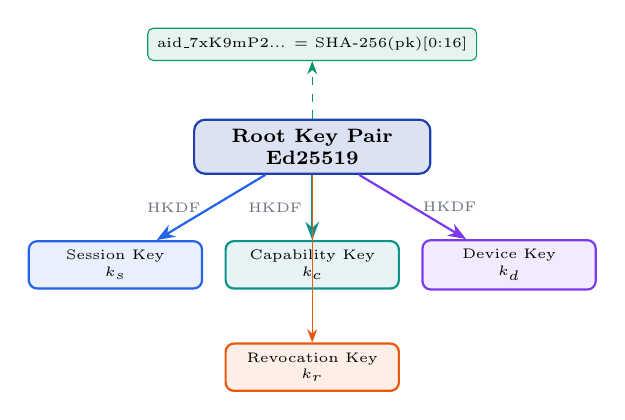
\begin{tikzpicture}[
  every node/.style={font=\scriptsize},
  rootbox/.style={rectangle, rounded corners=4pt, draw=aidarkblue, fill=aidarkblue!15, minimum width=3.0cm, minimum height=0.65cm, font=\scriptsize\bfseries, align=center, thick},
  keybox/.style={rectangle, rounded corners=3pt, draw=#1, fill=#1!10, minimum width=2.2cm, minimum height=0.5cm, font=\tiny, align=center, thick},
]
\node[rootbox] (root) at (0, 0) {Root Key Pair\\Ed25519};

\node[keybox=aiblue] (sess) at (-2.5, -1.5) {Session Key\\$k_s$};
\node[keybox=aiteal] (cap) at (0, -1.5) {Capability Key\\$k_c$};
\node[keybox=aipurple] (dev) at (2.5, -1.5) {Device Key\\$k_d$};

\node[keybox=aiorange] (rev) at (0, -2.8) {Revocation Key\\$k_r$};

\draw[-{Stealth}, aiblue, thick] (root) -- node[left, font=\tiny, text=aigray] {HKDF} (sess);
\draw[-{Stealth}, aiteal, thick] (root) -- node[left, font=\tiny, text=aigray] {HKDF} (cap);
\draw[-{Stealth}, aipurple, thick] (root) -- node[right, font=\tiny, text=aigray] {HKDF} (dev);
\draw[-{Stealth}, aiorange] (root) -- (rev);

% ID derivation
\node[rectangle, rounded corners=2pt, draw=aigreen, fill=aigreen!10, minimum width=2.4cm, minimum height=0.4cm, font=\tiny, align=center] (id) at (0, 1.3) {aid\_7xK9mP2... = SHA-256(pk)[0:16]};
\draw[-{Stealth}, aigreen, dashed] (root) -- (id);

\end{tikzpicture}
\caption{Identity anchor key hierarchy. The root Ed25519 key pair generates the permanent identity ID via SHA-256 truncation. Scoped child keys are derived via HKDF-SHA256 with structured context strings for session, capability, device, and revocation purposes.}
\label{fig:hierarchy}
\end{figure}

% ----------------------------------------------------------------------------
\subsection{Action Receipts}
\label{sec:receipts}

An action receipt is a signed cryptographic object that proves an agent took a specific action at a specific time. Every receipt contains the actor's identity (public key), the action type (decision, observation, mutation, delegation, revocation, or custom), a structured content payload, a SHA-256 hash of the action content, and an Ed25519 signature over the hash.

\textbf{Receipt IDs} follow the same pattern as identity IDs: $\text{id} = \texttt{arec\_} \| \text{base58}(\text{SHA-256}(\text{receipt})[0\!:\!16])$.

\textbf{Hash chaining.} Each receipt can optionally reference a previous receipt by ID, creating a tamper-evident chain analogous to a blockchain but without consensus overhead. The receipt hash incorporates the previous receipt's ID, so any modification to an earlier receipt invalidates all subsequent hashes in the chain. An agent's action history is thus a verifiable, append-only log.

\textbf{Witness signatures.} Receipts support optional co-signatures from witness identities. When Agent~A takes an action observed by Agent~B, B can add its own signature to A's receipt, creating multi-party non-repudiation. Each witness signature includes the witness identity, timestamp, and Ed25519 signature over the receipt hash.

\textbf{Verification.} Receipt verification extracts the actor's public key from the receipt, recomputes the receipt hash from the content fields, and verifies the Ed25519 signature. For chained receipts, the verifier additionally checks that each link's previous-receipt reference is consistent.

% Figure 3: Receipt chain
\begin{figure}[t]
\centering
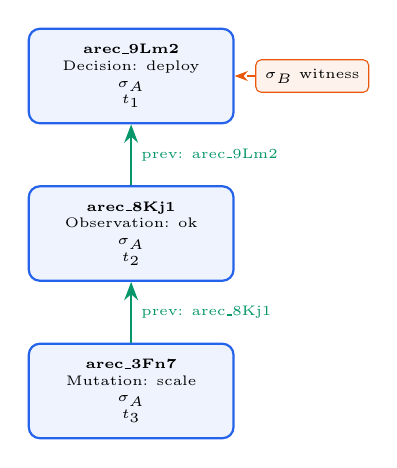
\begin{tikzpicture}[
  every node/.style={font=\scriptsize},
  receipt/.style={rectangle, rounded corners=4pt, draw=aiblue, fill=aiblue!8, minimum width=2.6cm, minimum height=1.2cm, font=\tiny, align=center, thick},
  witness/.style={rectangle, rounded corners=2pt, draw=aiorange, fill=aiorange!8, minimum width=1.2cm, minimum height=0.35cm, font=\tiny, align=center},
]
\node[receipt] (r1) at (0, 0) {\textbf{arec\_9Lm2}\\Decision: deploy\\$\sigma_{A}$ \\$t_1$};
\node[receipt] (r2) at (0, -2.0) {\textbf{arec\_8Kj1}\\Observation: ok\\$\sigma_{A}$ \\$t_2$};
\node[receipt] (r3) at (0, -4.0) {\textbf{arec\_3Fn7}\\Mutation: scale\\$\sigma_{A}$ \\$t_3$};

\draw[-{Stealth}, aigreen, thick] (r2) -- node[right, font=\tiny, text=aigreen] {prev: arec\_9Lm2} (r1);
\draw[-{Stealth}, aigreen, thick] (r3) -- node[right, font=\tiny, text=aigreen] {prev: arec\_8Kj1} (r2);

% Witness
\node[witness] (w1) at (2.3, 0) {$\sigma_{B}$ witness};
\draw[-{Stealth}, aiorange, dashed] (w1) -- (r1);

\end{tikzpicture}
\caption{Receipt chain structure. Each receipt contains the actor's signature and optionally links to a previous receipt via its ID, creating a tamper-evident audit trail. Witness co-signatures enable multi-party attestation.}
\label{fig:chain}
\end{figure}

% ----------------------------------------------------------------------------
\subsection{Trust Web}
\label{sec:trust}

A trust grant is a signed cryptographic object where Identity~A declares: ``I trust Identity~B to perform \{capabilities\} under \{constraints\}.'' Trust grants are the mechanism by which agents receive authority and are held accountable for its use.

\textbf{Capability URIs.} Permissions are expressed as structured URI strings with colon-delimited hierarchies: \texttt{read:calendar}, \texttt{execute:deploy:production}, \texttt{storage/write}. Wildcard matching is supported: a grant of \texttt{read:*} covers any capability prefixed with \texttt{read:}. The universal wildcard \texttt{*} grants full authority.

\textbf{Constraints.} Each grant carries a \texttt{TrustConstraints} structure specifying: \texttt{not\_before} (activation time), \texttt{not\_after} (expiration), \texttt{max\_uses} (count limit), and optional geographic or IP restrictions. Verification checks all constraints at query time.

\textbf{Delegation.} A grant can optionally allow the grantee to delegate authority to a third party. Delegation is controlled by two parameters: a boolean \texttt{delegation\_allowed} flag and an integer \texttt{max\_delegation\_depth}. If Agent~A grants to Agent~B with depth~3, then B can delegate to C (depth~1), C to D (depth~2), and D to E (depth~3), but E cannot further delegate. Each delegated grant references its parent grant ID and increments the depth counter.

\textbf{Revocation.} Every trust grant includes a \texttt{RevocationConfig} specifying a revocation key ID, a revocation channel (local, HTTP endpoint, or distributed ledger), and optional required witnesses. Revocation produces a signed \texttt{Revocation} record published to the configured channel. Verification checks revocation status before accepting any grant.

\textbf{Chain verification.} For delegated trust, verification walks the entire chain from root to terminal grant, checking at each link: (1)~signature validity, (2)~time constraints, (3)~revocation status, (4)~capability coverage (each delegated grant must be a subset of its parent's capabilities), and (5)~delegation depth within limits.

% Figure 4: Trust web example (full width)
\begin{figure*}[t]
\centering
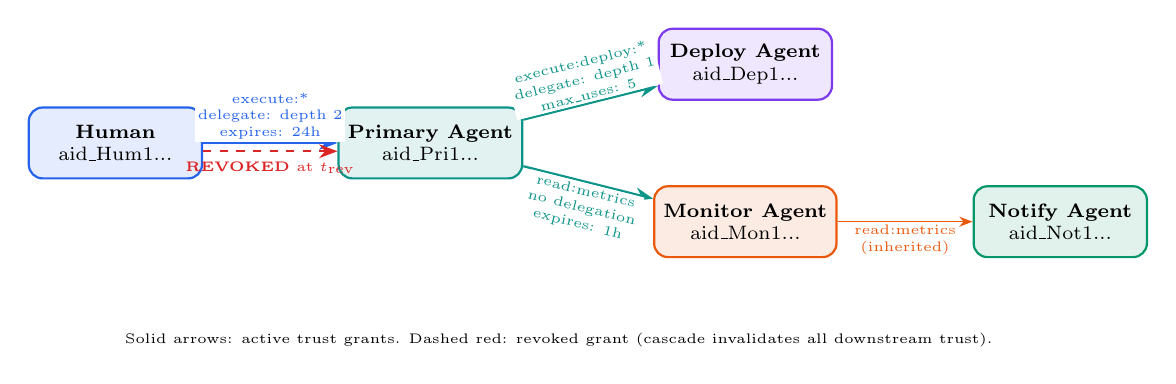
\begin{tikzpicture}[
  node distance=2.0cm,
  every node/.style={font=\small},
  idbox/.style={rectangle, rounded corners=5pt, draw=#1, fill=#1!12, minimum width=2.2cm, minimum height=0.9cm, font=\scriptsize, align=center, thick},
  grantlabel/.style={font=\tiny, align=center, text=#1, fill=white, inner sep=1pt},
]

\node[idbox=aiblue] (human) at (0, 0) {\textbf{Human}\\aid\_Hum1...};
\node[idbox=aiteal] (primary) at (4, 0) {\textbf{Primary Agent}\\aid\_Pri1...};
\node[idbox=aipurple] (deploy) at (8, 1) {\textbf{Deploy Agent}\\aid\_Dep1...};
\node[idbox=aiorange] (monitor) at (8, -1) {\textbf{Monitor Agent}\\aid\_Mon1...};
\node[idbox=aigreen] (notify) at (12, -1) {\textbf{Notify Agent}\\aid\_Not1...};

% Trust grants
\draw[-{Stealth}, aiblue, thick] (human) -- node[grantlabel=aiblue, above] {execute:*\\delegate: depth 2\\expires: 24h} (primary);
\draw[-{Stealth}, aiteal, thick] (primary) -- node[grantlabel=aiteal, above, sloped] {execute:deploy:*\\delegate: depth 1\\max\_uses: 5} (deploy);
\draw[-{Stealth}, aiteal, thick] (primary) -- node[grantlabel=aiteal, below, sloped] {read:metrics\\no delegation\\expires: 1h} (monitor);
\draw[-{Stealth}, aiorange] (monitor) -- node[grantlabel=aiorange, below] {read:metrics\\(inherited)} (notify);

% Revoked
\draw[-{Stealth}, aired, thick, dashed] ([yshift=-3pt]human.east) -- ([yshift=-3pt]primary.west) node[midway, below, font=\tiny, text=aired] {\textbf{REVOKED} at $t_{\text{rev}}$};

% Legend
\node[font=\tiny, anchor=west] at (0, -2.5) {Solid arrows: active trust grants. Dashed red: revoked grant (cascade invalidates all downstream trust).};

\end{tikzpicture}
\caption{Trust web example showing delegation from a human operator through a hierarchy of agents. The human grants \texttt{execute:*} to the primary agent with delegation depth~2. The primary delegates scoped subsets to deploy and monitor agents. When the root grant is revoked (dashed red), all downstream trust is automatically invalidated during verification.}
\label{fig:trustweb}
\end{figure*}


% ============================================================================
% 4. IMPLEMENTATION
% ============================================================================
\section{Implementation}
\label{sec:implementation}

AgenticIdentity is implemented in 10{,}859 lines of Rust organized as a Cargo workspace with four crates.

\textbf{Core library} (\texttt{agentic-identity}, 5{,}563~lines) provides the cryptographic primitives, data structures, storage layer, index engine, and query interface. Table~\ref{tab:primitives} lists the cryptographic algorithms used.

\begin{table}[t]
\caption{Cryptographic primitives used in AgenticIdentity.}
\label{tab:primitives}
\centering
\scriptsize
\begin{tabular}{@{}llll@{}}
\toprule
\textbf{Primitive} & \textbf{Algorithm} & \textbf{Purpose} & \textbf{Crate} \\
\midrule
Digital signature & Ed25519 & Identity, signing & ed25519-dalek \\
Key exchange & X25519 & Encrypted channels & x25519-dalek \\
Key derivation & HKDF-SHA256 & Scoped child keys & hkdf \\
Password KDF & Argon2id & Encrypted storage & argon2 \\
Sym.\ encryption & ChaCha20-Poly1305 & .aid file encryption & chacha20poly1305 \\
Hashing & SHA-256 & Receipt/grant hashes & sha2 \\
Memory safety & Zeroize & Private key clearing & zeroize \\
\bottomrule
\end{tabular}
\end{table}

The storage layer implements the \texttt{.aid} file format for encrypted identity persistence. Private keys are encrypted using a three-stage pipeline: the user's passphrase is processed through Argon2id~\cite{biryukov2016argon2} ($m\!=\!65536$~KiB, $t\!=\!3$ iterations, $p\!=\!4$ lanes) to derive a master key, which is expanded via HKDF-SHA256 into an encryption key, then used with ChaCha20-Poly1305~\cite{bernstein2008chacha} with a random 12-byte nonce. The public identity document is stored alongside in plaintext, enabling identity verification without decryption.

Receipt and trust stores are organized as directory trees of JSON files with in-memory indexes (HashMaps keyed by ID, actor, type; BTreeMaps for time-range queries). The query engine supports filtering by actor, type, time range, capability prefix, and validity status, with configurable sort order and result limits.

\textbf{CLI} (\texttt{agentic-identity-cli}, 1{,}121~lines) provides the \texttt{aid} binary with subcommands: \texttt{init}, \texttt{show}, \texttt{list}, \texttt{sign}, \texttt{verify}, \texttt{trust} (grant/revoke/list), \texttt{rotate}, \texttt{export}, and \texttt{receipt} (list). All commands support \texttt{--json} output for programmatic use.

\textbf{MCP server} (\texttt{agentic-identity-mcp}, 2{,}431~lines) implements the Model Context Protocol~\cite{mcp_spec_2024} over stdio with JSON-RPC~2.0 transport, exposing 10~tools (identity creation, action signing, receipt verification, trust management, health check) and 6~resources via \texttt{aid://} URI templates. The server enables any MCP-compatible LLM client---including Claude Desktop, VS~Code with Copilot, and Cursor---to manage agent identity through natural language tool invocations.

\textbf{FFI} (\texttt{agentic-identity-ffi}, 1{,}176~lines) provides 11~C-compatible functions with opaque pointer handles and numeric error codes, enabling integration from Python, Node.js, Go, and any language with C FFI support.

\textbf{Testing.} The implementation includes 182~tests across all crates: 143~in the core library covering cryptographic operations, identity lifecycle, receipt creation and verification, trust grant semantics, capability matching, storage persistence, indexing, and query filtering; 30~in the MCP server testing all tools and resources; and 9~in the FFI crate testing the complete C API surface.


% ============================================================================
% 5. EVALUATION
% ============================================================================
\section{Evaluation}
\label{sec:evaluation}

We evaluate AgenticIdentity along two dimensions: performance benchmarks to establish suitability for interactive agent systems, and security analysis to characterize the threat model and guarantees.

% ----------------------------------------------------------------------------
\subsection{Performance Benchmarks}
\label{sec:benchmarks}

\textbf{Hardware.} Apple~M4~Pro (ARM64), 48\,GB unified memory, macOS~15.

\textbf{Software.} Rust~1.86.0, compiled with \texttt{--release} (full optimizations). All benchmarks use the Criterion~\cite{criterion} statistical framework with 100~iterations per measurement and outlier detection.

Table~\ref{tab:benchmarks} reports the results. All operations complete in under 125\,\textmu{}s, well within the latency budget for interactive agent systems where tool calls typically take 100--500\,ms of network round-trip time.

\begin{table}[t]
\caption{Performance benchmarks (Apple M4 Pro, release mode, Criterion 100 samples). All operations are sub-millisecond.}
\label{tab:benchmarks}
\centering
\scriptsize
\begin{tabular}{@{}lr@{}}
\toprule
\textbf{Operation} & \textbf{Latency} \\
\midrule
Ed25519 key generation & 8.80\,\textmu{}s \\
Ed25519 sign & 9.17\,\textmu{}s \\
Ed25519 verify & 19.34\,\textmu{}s \\
HKDF key derivation & 972\,ns \\
\midrule
Identity anchor creation & 8.78\,\textmu{}s \\
Action receipt sign & 11.55\,\textmu{}s \\
Action receipt verify & 21.77\,\textmu{}s \\
\midrule
Trust grant sign & 12.41\,\textmu{}s \\
Trust grant verify & 21.84\,\textmu{}s \\
Trust chain verify (depth 2) & 43.51\,\textmu{}s \\
\midrule
Receipt chain (10 receipts) & 123.77\,\textmu{}s \\
\bottomrule
\end{tabular}
\end{table}

Several observations merit discussion. Key generation at 8.80\,\textmu{}s is dominated by the Ed25519 scalar multiplication on Curve25519; this is $>$100$\times$ faster than the 1\,ms target specified in our design requirements. Signing (9.17\,\textmu{}s) and verification (19.34\,\textmu{}s) exhibit the expected 2$\times$ asymmetry characteristic of Ed25519, where verification requires both scalar multiplication and point decompression.

Receipt signing (11.55\,\textmu{}s) adds only 2.38\,\textmu{}s over raw Ed25519 signing for SHA-256 hashing and JSON serialization of the action content. Trust grant verification (21.84\,\textmu{}s) is nearly identical to receipt verification, as both are dominated by the Ed25519 verify operation. Trust chain verification scales linearly with depth: at 43.51\,\textmu{}s for depth~2, we project depth~10 at $\sim$218\,\textmu{}s, well under the 5\,ms design target.

HKDF key derivation at 972\,ns is noteworthy: deriving a scoped child key adds less than 1\,\textmu{}s, making on-the-fly key derivation practical for every tool invocation.

% Figure 5: Benchmark bar chart
\begin{figure}[t]
\centering
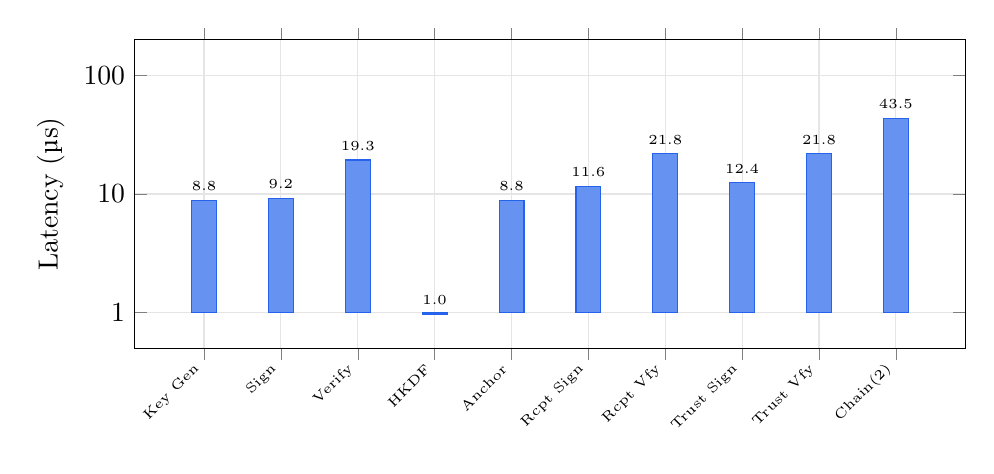
\begin{tikzpicture}
\begin{axis}[
  width=\columnwidth,
  height=5.5cm,
  ybar,
  bar width=9pt,
  xlabel={},
  ylabel={Latency (\textmu{}s)},
  ymode=log,
  log basis y=10,
  symbolic x coords={Key Gen, Sign, Verify, HKDF, Anchor, Rcpt Sign, Rcpt Vfy, Trust Sign, Trust Vfy, Chain(2)},
  xtick=data,
  xticklabel style={rotate=45, anchor=east, font=\tiny},
  ytick={0.1, 1, 10, 100},
  yticklabels={0.1, 1, 10, 100},
  ymin=0.5,
  ymax=200,
  grid=major,
  grid style={gray!20},
  nodes near coords,
  every node near coord/.append style={font=\tiny, anchor=south, rotate=0},
  point meta=explicit symbolic,
]
\addplot[fill=aiblue!70, draw=aiblue] coordinates {
  (Key Gen, 8.80) [8.8]
  (Sign, 9.17) [9.2]
  (Verify, 19.34) [19.3]
  (HKDF, 0.972) [1.0]
  (Anchor, 8.78) [8.8]
  (Rcpt Sign, 11.55) [11.6]
  (Rcpt Vfy, 21.77) [21.8]
  (Trust Sign, 12.41) [12.4]
  (Trust Vfy, 21.84) [21.8]
  (Chain(2), 43.51) [43.5]
};
\end{axis}
\end{tikzpicture}
\caption{Benchmark results on log scale. All operations complete in under 50\,\textmu{}s except 10-receipt chain creation (124\,\textmu{}s, not shown). HKDF derivation at $<$1\,\textmu{}s enables on-the-fly key scoping.}
\label{fig:benchmarks}
\end{figure}

% Throughput analysis
Table~\ref{tab:throughput} translates these latencies into throughput figures for capacity planning.

\begin{table}[t]
\caption{Throughput derived from benchmark latencies, assuming single-threaded operation.}
\label{tab:throughput}
\centering
\scriptsize
\begin{tabular}{@{}lr@{}}
\toprule
\textbf{Operation} & \textbf{Throughput} \\
\midrule
Identity creation & 113{,}895/s \\
Action signing & 86{,}580/s \\
Action verification & 45{,}936/s \\
Trust grant creation & 80{,}645/s \\
Trust verification & 45{,}787/s \\
Key derivation (HKDF) & 1{,}028{,}806/s \\
\bottomrule
\end{tabular}
\end{table}

% ----------------------------------------------------------------------------
\subsection{Security Analysis}
\label{sec:security}

\textbf{Threat model.} We assume the Dolev-Yao~\cite{dolev1983security} network attacker model: the adversary can intercept, modify, replay, and inject messages on any network channel. Private keys are assumed secure (protected by Argon2id-encrypted storage with zeroization~\cite{zeroize_crate} on drop). We do not address side-channel attacks on the host platform.

\textbf{Security properties.} AgenticIdentity provides the following guarantees:

\begin{enumerate}[nosep, leftmargin=*]
  \item \textbf{Identity binding.} An identity ID is cryptographically bound to its public key via SHA-256 truncation. Forging an ID requires finding a SHA-256 preimage, which is computationally infeasible at 128~bits.
  \item \textbf{Action non-repudiation.} A signed receipt proves the holder of the corresponding private key authorized the action. Under the assumption that private keys are not compromised, the actor cannot deny having taken the action.
  \item \textbf{Chain integrity.} Tampering with any receipt in a chain invalidates all subsequent receipt hashes. The chain provides the same integrity guarantee as a hash chain (blockchain without consensus).
  \item \textbf{Trust scoping.} Capability URI matching enforces that a grantee can only exercise permissions explicitly granted. Wildcard semantics are prefix-based: \texttt{read:*} matches \texttt{read:calendar} but not \texttt{write:calendar}.
  \item \textbf{Revocation completeness.} Revoking a root grant in a delegation chain invalidates all downstream grants during verification, because chain verification checks every link.
  \item \textbf{Key rotation continuity.} Key rotation preserves identity ID stability while the rotation record, signed by the old key, provides an authorization chain that verifiers can audit.
\end{enumerate}

Table~\ref{tab:security} summarizes the security properties and their cryptographic basis.

\begin{table}[t]
\caption{Security properties and their cryptographic foundations.}
\label{tab:security}
\centering
\scriptsize
\begin{tabular}{@{}lll@{}}
\toprule
\textbf{Property} & \textbf{Mechanism} & \textbf{Strength} \\
\midrule
Identity binding & SHA-256 $\to$ ID & 128-bit preimage \\
Non-repudiation & Ed25519 signature & 128-bit EUF-CMA \\
Chain integrity & SHA-256 hash chain & 256-bit collision \\
Key secrecy & Argon2id + ChaCha20 & 256-bit symmetric \\
Key derivation & HKDF-SHA256 & PRF security \\
Memory safety & Zeroize on drop & Prevents leak \\
\bottomrule
\end{tabular}
\end{table}

\textbf{Limitations.} AgenticIdentity does not address: (1)~time authority---timestamps are taken from the host clock and are not externally attested; (2)~key compromise recovery---if a root private key is extracted before rotation, the adversary can forge actions; (3)~anonymous credentials---every action is attributable to an identity, which may conflict with privacy requirements. These represent directions for future work (Section~\ref{sec:conclusion}).


% ============================================================================
% 6. USE CASES
% ============================================================================
\section{Use Cases}
\label{sec:usecases}

\textbf{Agent accountability.} When a coding agent deploys a breaking change to production, the signed receipt chain proves exactly which agent took which actions in what order. Incident response becomes a matter of cryptographic verification rather than log archaeology.

\textbf{Multi-agent coordination.} In a system where multiple agents collaborate---a planner, a coder, a reviewer, and a deployer---each agent's identity anchor enables mutual authentication. The planner grants \texttt{execute:code:*} to the coder with a 1-hour expiry; the coder grants \texttt{read:diff} to the reviewer; the reviewer grants \texttt{execute:deploy:staging} to the deployer. Every delegation is scoped, time-bounded, and revocable.

\textbf{Delegated authority with audit trails.} A human operator grants an executive agent broad authority (\texttt{execute:*}, delegation depth~3). The executive delegates scoped subsets to specialist agents. When the human revokes the root grant---perhaps because the executive's behavior deviated from expectations---all downstream trust is automatically invalidated. The full receipt chain provides a complete audit trail for post-mortem analysis.

\textbf{Cross-system portability.} An agent's \texttt{.aid} file is a self-contained portable identity. The agent can move between Claude Desktop, VS~Code, Cursor, or a custom MCP client without losing its identity, trust relationships, or action history. The MCP integration means any MCP-compatible tool can verify the agent's identity and check its authority before executing a request.


% ============================================================================
% 7. RELATED WORK
% ============================================================================
\section{Related Work}
\label{sec:related}

\textbf{SPIFFE/SPIRE}~\cite{spiffe_2024} is the closest infrastructure-level analog, providing workload identity for cloud services via X.509-SVIDs or JWT-SVIDs. SPIFFE identifies \emph{workloads}, not individual agent instances, and lacks per-action signing, receipt chains, and capability-scoped trust delegation. AgenticIdentity could complement SPIFFE by providing agent-level identity within a SPIFFE-authenticated service mesh.

\textbf{Decentralized Identifiers}~\cite{did_core_2022} provide a standards-based framework for self-sovereign identity. While DIDs could serve as an alternative identity layer, most DID methods require blockchain anchoring (adding latency and infrastructure dependencies) and the DID Document specification does not define action receipts or trust delegation semantics. A future version of AgenticIdentity could expose identities as DID documents for interoperability.

\textbf{Capability-based security}~\cite{dennis1966capabilities, miller2006capability} is a long-standing approach to access control where a ``capability'' is an unforgeable token granting specific rights. Macaroons~\cite{macaroons2014} extend this with contextual caveats that can attenuate authority. AgenticIdentity's trust grants are conceptually similar to attenuated macaroons with the addition of delegation chains, explicit revocation, and identity binding.

\textbf{Blockchain identity} systems~\cite{ethereum_erc725, hyperledger_indy} provide decentralized, tamper-evident identity registries. However, they introduce consensus latency (seconds to minutes), require gas fees or permissioned networks, and do not address per-action signing or scoped trust for AI agents. AgenticIdentity achieves tamper-evidence through hash chains without consensus overhead.

\textbf{AgenticOS ecosystem.} AgenticIdentity is the fourth module in the AgenticOS suite. AgenticMemory~\cite{owolabi2026agenticmemory} provides persistent cognitive memory via binary graph files. AgenticCodebase~\cite{owolabi2026agenticcodebase} provides semantic code navigation. AgenticVision~\cite{owolabi2026agenticvision} provides visual perception and persistent screenshots. AgenticIdentity provides the cryptographic trust layer that enables these modules to operate with accountability and verifiable authority.


% ============================================================================
% 8. CONCLUSION
% ============================================================================
\section{Conclusion}
\label{sec:conclusion}

We have presented AgenticIdentity, a cryptographic trust anchor that gives AI agents persistent, portable, mathematically verifiable identity. Through three interlocking primitives---identity anchors, action receipts, and a trust web---AgenticIdentity enables agent accountability, scoped trust delegation, tamper-evident audit trails, and cross-system portability, all without external service dependencies.

The implementation delivers strong performance in a compact footprint: 10{,}859 lines of Rust, 182~tests, four crates (core library, CLI, MCP server, FFI), and sub-50\,\textmu{}s latency for all individual cryptographic operations. Key generation at 8.80\,\textmu{}s, action signing at 11.55\,\textmu{}s, and trust verification at 21.84\,\textmu{}s confirm that cryptographic identity is practical for interactive agent systems where tool-call latency is measured in hundreds of milliseconds.

\textbf{Future work.} Three directions merit investigation. First, \emph{verifiable timestamps} via an external timestamping authority (RFC~3161) or trusted execution environment would strengthen non-repudiation. Second, \emph{selective disclosure}---enabling an agent to prove it holds a capability without revealing its full identity---would address privacy requirements in multi-tenant systems. Third, \emph{DID interoperability} would allow AgenticIdentity anchors to participate in broader decentralized identity ecosystems.

\textbf{Availability.} AgenticIdentity is open-source under the MIT license. The source code, documentation, benchmarks, and this paper are available at \url{https://github.com/agentralabs/agentic-identity}.

% ============================================================================
% REFERENCES
% ============================================================================
\bibliographystyle{plain}
\bibliography{references}

\end{document}
